\section[Single Row Functions]{Single Row Functions}
\hrulefill
\begin{itemize}
    \item Retrieve the email domain for the admin with Admin\_ID = 1
\end{itemize}

\begin{lstlisting}[caption={ Query 1},label={lst:q-1}]
    SELECT Admin_Email, SUBSTR(Admin_Email, INSTR(Admin_Email, '@') + 1) AS Email_Domain
    FROM Admin
    WHERE Admin_ID = 1;
\end{lstlisting}

\begin{figure}[H]
    \centering
    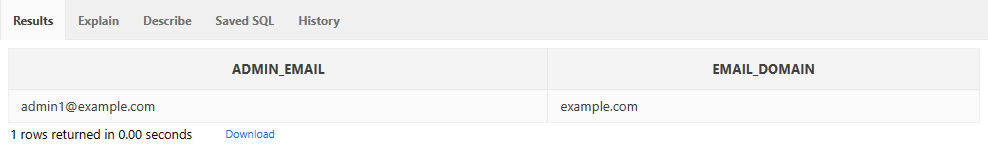
\includegraphics[width=1\textwidth]{images/dml/Q1.png}
    \caption{Result of Query 1}
\end{figure}
\clearpage
% % %

\begin{itemize}
    \item Get the hire date of the manager named 'John Doe' formatted in a specific way
\end{itemize}
\begin{lstlisting}[caption={ Query 2},label={lst:q-2}]
    SELECT Manager_Name, TO_CHAR(Manager_Hiredate, 'DD-Mon-YYYY') AS Hire_Date
    FROM Manager
    WHERE Manager_Name = 'John Doe';
\end{lstlisting}

\begin{figure}[H]
    \centering
    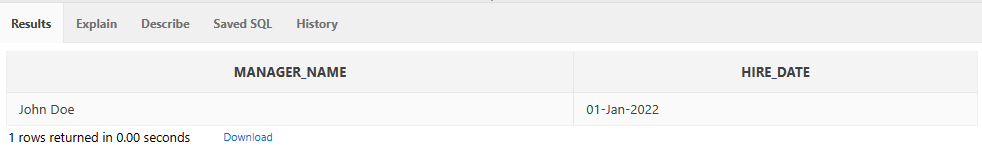
\includegraphics[width=1\textwidth]{images/dml/Q2.png}
    \caption{Result of Query 2}
\end{figure}

%%%
\begin{itemize}
    \item Concatenate the first and last name of the content creator with ContentCreator\_ID = 1
\end{itemize}
\begin{lstlisting}[caption={ Query 3},label={lst:q-3}]
    SELECT ContentCreator_Name, CONCAT(CONCAT(SUBSTR(ContentCreator_Name, 1, INSTR(ContentCreator_Name, ' ') - 1), ' '), SUBSTR(ContentCreator_Name, INSTR(ContentCreator_Name, ' ') + 1)) AS Full_Name
    FROM ContentCreator
    WHERE ContentCreator_ID = 1;
\end{lstlisting}

\begin{figure}[H]
    \centering
    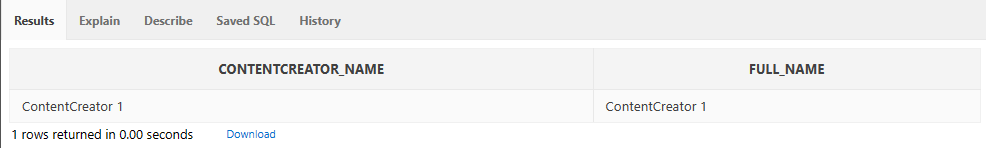
\includegraphics[width=1\textwidth]{images/dml/Q3.png}
    \caption{Result of Query 3}
\end{figure}
